\chapter{Background and Related Work}
\label{ch:related}

One of the most cited and comprehensive articles out there for getting to know the field of fairness in machine learning is the survey paper by \citet{Mehrabi:2021:CSUR}. This paper elaborates numerous concerns about the fairness of the models’ outputs. It serves as a gateway to a lot of the current research in the field, a lot of which will be summarised in this section of the thesis.

\section{Algorithmic Fairness}

Many definitions of discrimination exist, and while there is no gold-standard, it is often defined as an absence of any prejudice or favouritism towards individuals or groups based on some intrinsic traits \cite{Mehrabi:2021:CSUR, Nripsuta:2019:AIES}. These definitions are core in the many mathematical definitions of fairness. Some of these are summarised below

\textbf{Equalized Odds}: According to \citet{Mehrabi:2021:CSUR, Hardt:2016:NIPS} A predictor $\hat{Y}$ satisfies equalised odds with respect to a sensitive attribute $A$ and outcome $Y$ if $\hat{Y}$ and $A$ are conditionally independent on $Y$. i.e.

\begin{equation*}
    P(\hat{Y}|A=0, Y=y) = P(\hat{Y}|A=1, Y=y), y \in {0, 1}
\end{equation*}

\textbf{Equal Opportunity}: According to \citet{Mehrabi:2021:CSUR, Hardt:2016:NIPS} A binary predictor $\hat{Y}$ satisfies equal opportunity with respect to $A$ and $Y$ if

\begin{equation*}
    P(\hat{Y}=1|A=0, Y=1) = P(\hat{Y}=1|A=1, Y=1)
\end{equation*}

\textbf{Demographic Parity}: According to \citet{Mehrabi:2021:CSUR, Dwork:2012:ITCS} A predictor $\hat{Y}$ satisfies demographic parity if 

\begin{equation}
    P(\hat{Y}|A=0) = P(\hat{Y}|A=1)
    \label{eq:dempar}
\end{equation}

And many more metrics exist. A challenge is that according to \citet{Mehrabi:2021:CSUR, Kleinberg:2017:LIPIcs} it is impossible to satisfy some of these fairness constraints. One should therefore be considerate when using a certain metric. Synthesising these definitions to one gold-standard remains an open RQ. For this thesis. Demographic parity is especially important as it is fundamental to the model described in Section~\ref{sec:paper1}.

\textbf{Strong Demographic Parity}: According to \citet{Antonio:2021:arXiv}, this is a parity score that extends demographic parity by considering fairness throughout the entire range of possible decision thresholds. It was proposed by \citet{Jiang:2020:PMLR}. When learning a fair classifier to satisfy strong demographic parity, the predictor $\hat{Y}$ must satisfy demographic parity for any threshold $t$ and sensitive attribute $A$

$$
\forall t \in \hat{Y} : P(\hat{Y} \geq t | A = 0) = P(\hat{Y} \geq t | A = 1)
$$

This assumes that the model output $\hat{Y}$ is a probability or score of belonging to the class of interest and $t$ is a selected threshold for classifying.

\section{Methods for Fair Machine Learning}

Machine Learning is a large domain, encompassing many subdomains. These include \textit{Classification, Regression, PCA, Clustering, Deep Learning} and many more. In this thesis, the focus will be on fair classification. 

\textit{Fair Classification:} Some of the most important works in the field of fair classification are summarised by \cite{Mehrabi:2021:CSUR}. Of special importance for this thesis is the naïve Bayes approach for fair classification by \citet{Calders:20210:DMKD} In this work the authors investigated how to modify the naïve Bayes classifier in order to perform classification that is independent of the sensitive attributes. In this paper they measure discrimination by \textit{discrimination score} which is defined as

\begin{equation*}
    P(C=+|S_+) - P(C=+|S_-)
\end{equation*}

Which assumes that a classifier is fair if the outcome is independent of the sensitive attribute. i.e., \textit{Demographic Parity} as described above. The main limitation of this paper is that the classifier on the non-sensitive attributes is a naïve Bayes classifier. This means it assumes that all the features are independent. This makes it one of the simplest Bayesian networks out there as well as scalable since the number of parameters scales linearly with the number of features. We address this limitation further in Section~\ref{sec:probmac}.

Other important works are the works of \cite{Zafar:2017:NIPS} and \citet{Dwork:2018:PMLR}. \citet{Zafar:2017:NIPS} introduced new notions on how to define fairness, arguing that the traditional parity based notion is  quite stringent, limiting the overall decision-making accuracy. They tie in elements from envy-freeness literature in economics and game theory and propose preference-based notions of fairness. 

\citet{Dwork:2018:PMLR} provide a simple and efficient decoupling technique, which can be added on top of any black-box machine learning algorithm, to learn different classifiers for different groups. Using transfer learning to mitigate the problem of having too little data on any one group.

Important to this thesis is the work of \citet{Choi:2021:AIII} Which is a follow-up paper to \cite{Calders:20210:DMKD}. They have generalised the limitation of the first paper, where a naïve Bayes classifier was necessary. Their framework can be generalised to any local probabilistic network. This will be described in more detail in section \ref{sec:fairbayesiannetwork}. The work of \citet{Antonio:2021:arXiv} and their development of a fair tree based classifier using strong demographic parity is also important for this thesis and is described in more detail in section~\ref{sec:fairtree}.

\section{Probabilistic Machine Learning}
\label{sec:probmac}

In this thesis, we will focus on probabilistic machine learning, therefore a brief introduction to this field is in place. According to \citet{Murphy:2012:Book}, machine learning is usually divided into two main types. In \textbf{Predictive} or \textbf{Supervised learning} approach, the goal is to learn a mapping from inputs $x$ to outputs $y$ given a labelled set of input-output pairs \cite[p.~2]{Murphy:2012:Book}

\begin{equation*}
    \mathcal{D} = {(x_i, y_i)}_{i=1}^N
\end{equation*}

The second type is the \textbf{descriptive} or \textbf{unsupervised learning} where we are only given the data itself without labels

\begin{equation*}
    \mathcal{D} = {x_i}_{i=1}^N
\end{equation*}

here the goal is to find interesting patterns in the data that are inherent to the data itself without the need for labels. This problem is not as well-defined as the predictive case, and there is no obvious error metric. The third type is \textbf{reinforcement learning}, where you let an agent explore a space and reward desired behaviour through a performance or reward metric. 

A common way to perform supervised learning is to treat  $y$ as a random variable and estimate a mapping 

\begin{equation*}
    f: x \rightarrow y
\end{equation*}

One example of this is Linear Regression. Which maps input vectors $x$ to outputs $y$ using the following mapping \cite[p.~19]{Murphy:2012:Book}

\begin{equation*}
    f: y = \mathbf{w}^Tx + \epsilon = \sum_{j=1}^N w_j x_j + \epsilon
\end{equation*}

and often $\epsilon$ is assumed to be Gaussian and the model can be rewritten as 

\begin{equation*}
    p(y|x, \theta) = \mathcal{N}(y|\mu(x), \sigma^2(x))
\end{equation*}

One common way to estimate the parameters of a statistical model is to calculate the maximum likelihood estimate of the model parameters \cite[p.~217]{Murphy:2012:Book}

\begin{equation*}
    \hat{\mathbf{\theta}} = \argmax_{\theta} \log p(\mathcal{D}|\theta)
\end{equation*}

and for linear regression, minimising the sum of squared errors has an explicit solution \cite[p.~220]{Murphy:2012:Book}

\begin{equation*}
    \hat{\bf{w}}_{\text{OLS}} = (\bf{X}^T\bf{X})^{-1}\bf{X}^T\bf{y}
\end{equation*}

This estimate gives us a point estimate of the model parameters. This is traditionally what many machine learning algorithms do, take a dataset and calculate the most likely point estimate of the model parameters. It is reasonable to assume that the model parameters that are returned from one dataset are different to the true model parameters, and it would in many cases be beneficial to know how uncertain the model parameters are. This is where the \textbf{probabilistic} approach comes in.

In a probabilistic approach, we treat the input data and labels as random variables, but also the model parameters. After training, we will have a distribution of model parameters which we can sample from and simulate different realisations of our models. One example of this is \textbf{Bayesian Linear Regression}

In Bayesian linear regression, the likelihood of $y$ is given by \cite[p.~232]{Murphy:2012:Book}

\begin{equation*}
    p(\bf{y}|\bf{X}, \bf{w}, \mu, \sigma^2) = \mathcal{N}(\bf{y}|\mu + \bf{X}\bf{w}, \sigma^2 \bf{I}_N)
\end{equation*}

and using a Gaussian prior distribution since it is a conjugate prior, the posterior becomes \cite[p.~232]{Murphy:2012:Book}

\begin{equation*}
    p(\bf{w}|\bf{X}, \bf{y}, \sigma^2) \propto \mathcal{N}(\bf{w}|\bf{w_0}, \bf{V_0}) \mathcal{N}(\bf{y}|\bf{Xw}, \sigma^2\bf{I})
\end{equation*}

And we have a full distribution of model parameters, which gives us insight into the uncertainty of the model. This property is desired for assessing fairness and uncertainty later in this thesis.

\section{Graphical Models}

A graphical model is a way to represent a joint probability distribution. Nodes represent random variables and the edges between the random variables represent dependencies, and the lack of edges means the random variables are conditionally independent \cite[p.~308]{Murphy:2012:Book}. There are many graphical models, and all of them tie probability theory and graph theory together comprehensively. We describe some different models in this section.

\section{Bayesian Networks}

\begin{figure}[h!]
    \centering
    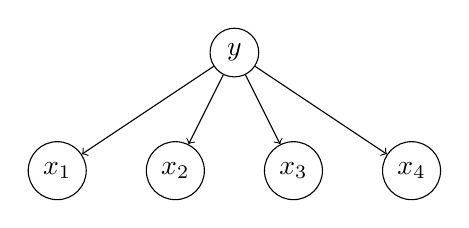
\begin{tikzpicture}[nodes={draw, circle}, ->]
        \node {$y$}
            child {node {$x_1$}}
            child {node {$x_2$}}
            child {node {$x_3$}}
            child {node {$x_4$}};
    \end{tikzpicture}
    \caption{Bayesian network with $4$ features representing the naïve Bayes classifier}
    \label{fig:my_label}
\end{figure}

Graphical models give us a graphical way to represent the joint PDF. It models the conditional dependencies between random variables. From this graph, we see that the joint probability distribution of this classifier is

\begin{equation*}
    p(y, x_1, x_2, x_3, x_4) = p(y)p(x_1|y)p(x_2|y)p(x_3|y)p(x_4|y)
\end{equation*}

\subsection{Naïve Bayes Classifier: Baseline Method}
\label{relatedwork:naiveBayes}
The naïve Bayes classifier is the simplest Bayesian network, assuming that all features are independent conditionally on the class variable, hence the name naïve Bayes. This naïve assumption gives the model few parameters to learn, and it requires little training data to achieve good performance. From the work by \citet{Zhang:2004:AAAI} we know that naïve Bayes classifiers perform well despite the assumption of independence among features due to the dependencies cancelling each other out and dependencies distributing evenly among classes.

According to \citet[p.~217]{Ankan:2015:Book}, assume that we have a dataset $X = (x_1, x_2, \dots, x_N)$ with $N$ independent features and $k$ classes $C_k$ that we want to classify the data to. naïve Bayes does this by modelling the posterior distribution in terms of the joint probability

$$
P(C_k | X) \propto P(C_k , X) = P(C_k) \prod_{i=1}^{n} P(x_i|C_k)
$$

Where the naïve assumption is that $P(x_i | X \setminus x_i , C_k) = P(x_i | C_k)$ i.e., the features are mutually independent conditioned on $C_k$. Different naïve Bayes methods exist for the assumptions on the priors and likelihoods, i.e. if they are Gaussian, binomial, categorical etc. The model classifies the data to the class that has the highest posterior probability. 

\subsection{pgmpy: naïve Bayes}

We have used the naïve Bayes classifier implemented in pgmpy and is used as a baseline method in the experiment described in section~\ref{sec:AdultFairnessAssessment}. The implementation in pgmpy implements a naïve Bayes method and assumes categorical distributions on all parameters. We calculated the probabilities as conditional probability tables (CPD Tables) using the MLE estimate from data. I.e. calculating probabilities from the dataset by counting occurrences conditioned on the class label. For more detail on how this is implemented, see pgmpy's documentation \footnote{\url{https://pgmpy.org/index.html}}.

\subsection{Structure Learning: Hill Climb Search}
\label{HillClimbSearch}
According to \citet[p.~811]{Koller:2009:Book} finding a maximum-score graphical network evaluated under any decomposable scoring function is NP-hard. Thus, we have to resort to a heuristic algorithm that attempt to find the best network, but are not guaranteed to do so. We have used Hill-Climb search which try to find the best graph $G_{\text{best}}$ by selecting an initial network $G_{\emptyset}$, which in pgmpy is a network with no edges. Then we search through all possible search operations $O$ to the network (delete, add, reverse in pgmpy) and score them. We perform the change that gives the best score until convergence or the maximum number of iterations is reached. The algorithm is shown below:

\begin{algorithm}
    \caption{Hill Climb Searched with Data Perturbation}
    \begin{algorithmic}
        \REQUIRE $G_{\emptyset} = $ Initial Network, $D = $ fully observed dataset, score $ = $ scoring function, $O = $ search operations, search $ = $ search procedure, $t_0 = $ initial perturbation size, $\gamma = $ Reduction in perturbation size.
        \ENSURE $G_{\text{best}} = $ Best network structure found.
        \STATE $G \leftarrow$ Search$(G_{\emptyset}, D, \text{Score}, O)$ 
        \STATE $G_{\text{best}} \leftarrow G$
        \STATE $t \leftarrow t_0$
        \FOR{$i \in \{ 1, \dots, \text{until convergence} \}$} 
        \STATE $D' \leftarrow $ Perturb$(D,t)$
        \STATE $G \leftarrow$ Search$(G, D', \text{Score}, O)$
        \IF{Score$(G : D) > \text{Score}(G_{\text{best}} : D)$}
            \STATE $G_{\text{best}} \leftarrow G$
        \ENDIF
        \STATE $t \leftarrow \gamma \cdot t$
        \ENDFOR
    \end{algorithmic}
\end{algorithm}

For more information about the algorithm and Hill Climb Search, see \cite[p.~816--819]{Koller:2009:Book} and the implementation in pgmpy which also adds some parameters like red-listed edges and non-changable edges.\footnote{\url{https:/Z/pgmpy.org/_modules/pgmpy/estimators/HillClimbSearch.html\#HillClimbSearch.estimate}}

\subsection{Parameter Learning: Expectation Maximization}
\label{Expectation Maximization}
After we have learned the model structure, we will have to learn the parameters of the model given its structure. Since we will use a model with latent variables, Expectation Maximisation is the algorithm of choice. The expectation maximisation algorithm in general as described by \citet{Murphy:2012:Book, Bishop:2006:Book} is as follows:

Consider a probabilistic model in which we collectively denote all the observed
variables by $\boldsymbol{X}$ and the latent variables $\boldsymbol{Z}$. The joint distribution $p(\boldsymbol{X}, \boldsymbol{Z} | \boldsymbol{\theta})$ is governed by the parameters $\boldsymbol{\theta}$. We want to maximise the likelihood given by

\begin{equation*}
    p(\boldsymbol{X} | \boldsymbol{\theta}) = \sum_{\boldsymbol{X}} p(\boldsymbol{X}, \boldsymbol{Z} | \boldsymbol{\theta})
\end{equation*}

Which is not computable, as $\boldsymbol{Z}$ is unknown. Therefore the expectation step is introduced which is to compute $Q$

\begin{equation*}
    Q(\boldsymbol{\theta, \theta^{\text{old}}}) = E[\log L(\boldsymbol{\theta}; \boldsymbol{X}, \boldsymbol{Z})]
\end{equation*}

In the M step we optimise $Q$ w.r.t. $\boldsymbol{\theta}$

\begin{equation*}
    \boldsymbol{\theta^{\text{new}}} = \argmax_{\boldsymbol{\theta}} Q(\boldsymbol{\theta, \theta^{\text{old}}})
\end{equation*}

this is done iteratively until a certain threshold is achieved. For more details on how exactly this is implemented in pgmpy, see the documentation.\footnote{\url{https://pgmpy.org/_modules/pgmpy/estimators/EM.html\#ExpectationMaximization}}

\section{Modelling Discrimination Process}
\label{sec:paper1}
Now that probabilistic machine learning and graphical models have been introduced, it is time to introduce the work of \citet{Choi:2021:AIII} in more detail. As discussed previously in this section. There are many sources of bias in data and it is reasonable to assume that almost all datasets out there is biased \citet{Choi:2021:AIII}. describes a way of learning fair probability distributions from biased data by explicitly modelling a latent variable that represents a hidden, unbiased label. In particular, they aim to achieve demographic parity by enforcing
certain independencies in the learned model.

\begin{figure}[h!]
    \centering
    \begin{tikzpicture}[nodes={draw, circle}, ->]
        \node (S) {$S$};
        \node (Df) [right=of S] {$D_f$};
        \node (X)  [below=of S] {$X$};
        \node (D)  [below=of Df] {$D$};
        
        \draw (S) -> (X);
        \draw (S) -> (D);
        \draw (Df) -> (X);
        \draw (Df) -> (D);
    \end{tikzpicture}
    \caption{Bayesian network structures that represent the proposed
fair latent variable approach from \cite{Choi:2021:AIII}}
    \label{fig:choinetwork}
\end{figure}

In other words, they model the process on how biased datasets are generated. The biased labels present in the dataset are dependent on the sensitive attributes $S$ and the true fair labels $D_f$. The latent variable $D_f$ is used for decision making on future instances by inferring $P(D_f|e)$ given some evidence.

The paper states that any probabilistic model can be used but that this model needs to satisfy the independence assumptions in the Bayesian network.

\section{Fair Tree Classifier}
\label{sec:fairtree}

The paper by \citet{Antonio:2021:arXiv} has been implemented in this thesis and the related python module. They introduce a new splitting criterion that evaluates splits in terms of the Area under curve (AUC) w.r.t. the predicted value and the sensitive attribute. Assume that we want to learn a classifier $f$ that learns a mapping from features $X$ and predictor $\hat{Y}$ which outputs a probability of belonging to the predicted class

$$
f: X \rightarrow \hat{Y}
$$

The AUC for this predictor w.r.t. the true labels $Y$ can be calculated as

\begin{equation*}
    AUC_Y(\hat{Y}, Y) =  \frac
    {
        \sum_{t_0 \in Y_{-}} \sum_{t_1 \in Y_{+}}  \textbf{1}[\hat{Y}_{t_0} < \hat{Y}_{t_1}]
    }
    {
        |Y_{-}| \cdot |Y_{+}|
    }
\end{equation*}

where $Y_-$ and $Y_+$ are the set of indexes for negative and positive instances in the true labels. $\textbf{1}$ denotes the indicator function. The authors calculate the AUC score for the predicted labels using scikit-learn \cite{Pedregosa:2011:JMLR} and the method called roc\_auc\_score \cite{Buitinck:2013:PKDD}. When calculating the AUC w.r.t. the sensitive attribute, denoted $AUC_s$ the authors have derived the following formula

\begin{equation}
    AUC(\hat{Y}, S) = \max(1 - AUC(\hat{Y}, S), AUC(\hat{Y}, S))
\end{equation}

The max operator maps the bounds to the range $[0.5, 1]$. The authors then introduce the splitting criterion used in their tree algorithm, Splitting Criterion AUC for Fairness (SCAFF). Which is calculated as

\begin{equation*}
    SCAFF(\hat{Y}, Y, S, \Theta) = (1 - \Theta) \cdot AUC_Y(\hat{Y}, Y) - \Theta \cdot AUC_S(\hat{Y}, S)
\end{equation*}

$\Theta$ is here a hyperparameter of the tree classifier. When $\Theta = 1$ splits are only evaluated in terms of fairness and vice versa.  As is typical with tree learning, the architecture is learned by evaluating splits at each depth and selecting the split that maximises the splitting criterion. Other hyperparameters as maximum depth, number of bins etc are also used.

\section{Interpretable Machine Learning}

Up until this point in the thesis, we have discussed fair machine learning models and sources of bias in the data. Another important field in machine learning that is important regarding fairness is Interpretable Machine Learning. Many methods for fairness rely on either pre-processing of the datasets to make the datasets more fair or in-processing methods that change the machine learning algorithm to reduce discrimination during training \cite{Mehrabi:2021:CSUR}.

Interpretable Machine Learning methods instead focus on understanding the mechanisms behind the decision that the machine learning model makes. This way, we can investigate how the machine learning model uses the data to make a prediction. According to \citet{Miller:2019:AIJ} interpretability is how well a human could understand the decisions in the given context. The notion of interpretability is domain-specific and depends on the purpose of the interpretable component in the first place. The higher the interpretability of a machine learning model, the easier it is for someone to comprehend why certain decisions or predictions have been made \cite{Molnar:2020:Book}.

\subsection{Example of interpretability}

Examples of interpretable machine learning models are Linear Regression, Logistic Regression and Decision Trees among many others. Linear Regression is especially interpretable, as we shall describe in this section. According to \citet{Molnar:2020:Book}, linear models can be used to model the dependence of a regression target $\boldsymbol{y}$ on some features $\boldsymbol{x}$. The learned relationships are linear and can be written for a single instance i as follows

\begin{equation*}
    \boldsymbol{y} = \boldsymbol{X} \boldsymbol{\beta} + \epsilon
\end{equation*}

Where $\beta_1$ is the weight associated with feature $X_1$. These weights can be interpreted in several ways depending on the nature of the feature.

\begin{itemize}
    \item Numerical Features: Increasing the feature by a unit of one increases the estimated outcome by $\beta_i$.
    \item Binary Feature: Changing the binary feature form the reference category to other category increases the outcome by $\beta_i$
    \item Categorical Feature: Create dummy variables. Interpretation of each dummy variable is the same as for binary features.
\end{itemize}

As you see, linear regression models are structured in such a way that it is easy to explicitly describe how the predictions of the models are made. Other models are also interpretable, which is described in more detail by \citet{Molnar:2020:Book}.